\section{Create a Branch to start making changes\label{sec:maintain_repo}}

This section covers how to create a branch and the importance of the naming convention that is used to track all the development. 

If you are using git client from a command prompt then creating a branch is easy by using the following command \texttt{git -b <BranchLabel>}. The \texttt{BranchLabel} has a specific naming convention, which is  \texttt{BranchLabel \ = \ simpledescription\_YYYYMM}. For example \texttt{git -b SplineSelectivity\_202307} which is adding or fixing the spline selectivity class which started in July of 2023. This makes it easier for the development team what is in the branch and how active it is.

Once you have created a branch you can switch between the master and branch using the \texttt{git checkout} command. To find out how to merge changes from the master into your branch just google \enquote{git merging master into feature branch} and you will find many useful resources.

Once you do your first push to the branch it you will then be able to see it under the branches tab on the online master repository (See Figure~\ref{fig:branchtab}). If you have trouble pushing the branch you may need one of the \CNAME\ developers to add you as a collaborator to the project. This would mean someone has to log into the NIWAFisheries GitHub account and go to settings tab of the \CNAME\ repository and add the user as a collaborator.

\begin{figure}[!ht]
	\centering
	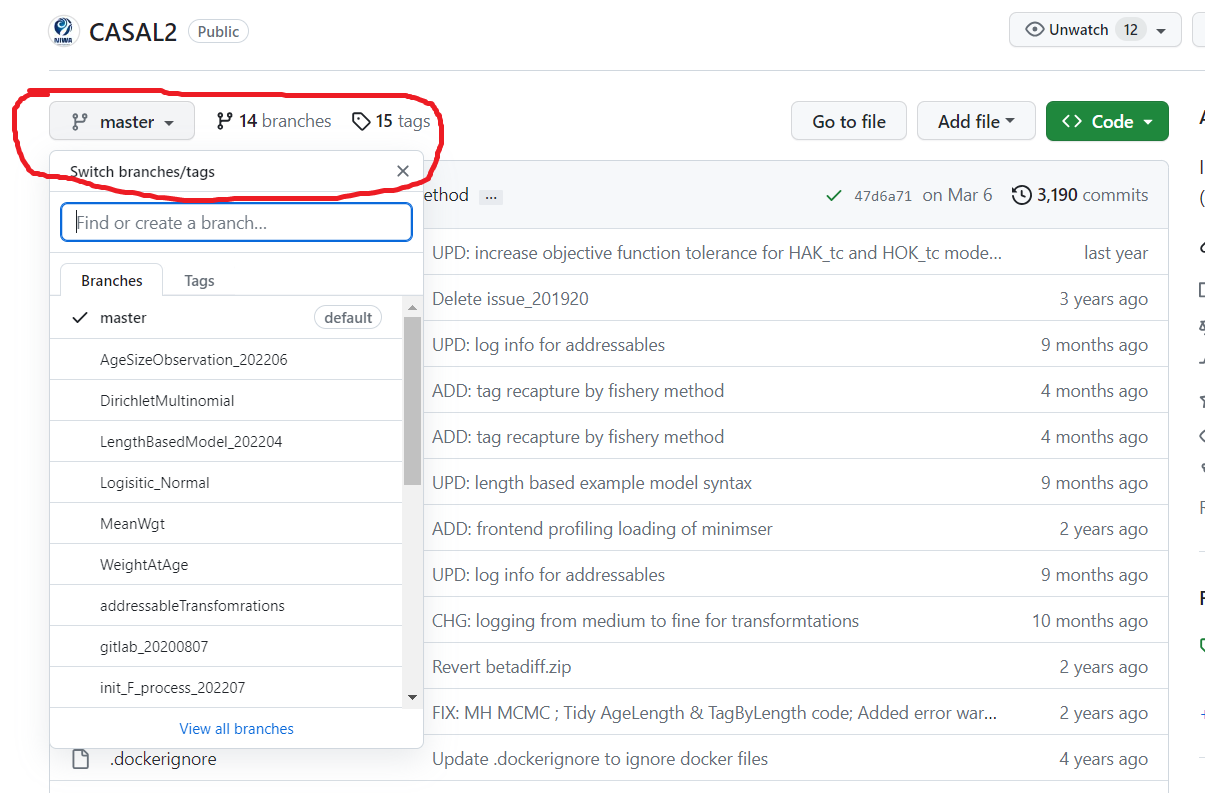
\includegraphics[scale=0.6]{Figures/branch_tab.png}
	\caption{}\label{fig:branchtab}
\end{figure}